\chapter{Systems Based on Chord}
Chord's efficient and scalable architecture has inspired the development of various systems and applications in the field of distributed computing and \gls{p2p} networks.
These systems leverage the unique properties of Chord's \gls{dht} to achieve robustness, fault tolerance, and efficient resource discovery.
This chapter explores several notable applications of Chord in different domains, highlighting real-world examples, advantages, disadvantages, and additional details.

\section{File Sharing Systems}
One of the most common applications of Chord is in file-sharing systems.
These systems use Chord's \gls{dht} to store and retrieve files efficiently, ensuring high availability and fault tolerance.
The \gls{cfs} employs Chord to provide a robust and efficient file storage and retrieval service.
It distributes file blocks across multiple nodes, ensuring redundancy and fault tolerance, making it suitable for large-scale file distribution.
\gls{cfs} breaks files into smaller chunks and distributes them across the network to balance the load and enhance data availability.
This approach not only improves access times but also ensures that the system can recover quickly from node failures, maintaining the integrity and availability of stored files (\cite{Dabek2001}).
Large-scale academic repositories and research data sets often use systems similar to \gls{cfs} to ensure data availability and fault tolerance.
The primary advantages of \gls{cfs} include high redundancy, fault tolerance, decentralized control, and scalability.
However, it can suffer from potentially high latency for file retrieval if the network is large or nodes are widely dispersed.

Ivy, a multi-user read/write \gls{p2p} file system, uses Chord for efficient data location, allowing users to collaboratively manage and share files in a decentralized manner (\cite{Ivy2003}).
Ivy supports concurrent file updates and conflict resolution, making it suitable for collaborative environments.
By leveraging Chord's \gls{dht}, Ivy can efficiently locate and manage file metadata, ensuring that users can quickly access the files they need.
This system exemplifies how Chord can be used to build robust, scalable file-sharing solutions that operate without central control.
Ivy-like systems are useful for collaborative projects in distributed teams, such as software development or content creation.
Ivy's main advantages are its support for collaborative file management, efficient metadata handling, and decentralized architecture.
However, conflict resolution can be complex, and there can be potential data inconsistency issues.

\section{Distributed Databases}
Chord's principles have been applied to the design of distributed databases, providing scalable and fault-tolerant data storage solutions.
Dynamo, developed by Amazon, is a distributed key-value store that uses concepts similar to Chord for partitioning and replicating data across multiple nodes.
Dynamo ensures high availability and durability, even in the presence of node failures.
It employs a consistent hashing mechanism to distribute data evenly across nodes, reducing hotspots and ensuring efficient load balancing.
Dynamo's replication and quorum-based techniques allow it to achieve high fault tolerance, making it a cornerstone of Amazon's highly available services (\cite{DeCandia2007}).
Amazon's Dynamo is the core of many of its services, ensuring consistent performance during events like Black Friday sales.
The primary advantages of Dynamo include high availability, fault tolerance, efficient load balancing, and scalability.
However, managing consistency and conflict resolution can be complex, and there is a high overhead for replication and quorum maintenance.

Cassandra is another highly scalable distributed database that employs a Chord-like \gls{dht} for data distribution.
It provides a decentralized and fault-tolerant architecture, making it suitable for large-scale applications.
Cassandra's architecture allows it to handle large amounts of data across many commodity servers, providing high throughput and low latency.
The use of Chord-like principles ensures that data is evenly distributed, enabling efficient query processing and robust data replication (\cite{Lakshman2010}).
Cassandra is used by companies like Facebook, Instagram, and Netflix to manage large-scale data requirements with high availability and low latency.
Its advantages include high scalability, low latency, fault tolerance, and a decentralized architecture.
However, Cassandra's complexity in data modeling and its eventual consistency model can lead to temporary data inconsistency.

\section{\acrlong{cdn}}
Chord's efficient resource discovery and routing capabilities make it a suitable choice for content distribution networks.
Coral is a content distribution network that uses Chord to locate and distribute web content efficiently.
It reduces the load on origin servers and enhances the scalability of content delivery.
By caching web content at various nodes across the network, Coral can quickly serve content to users from the nearest available node, reducing latency and improving user experience.
The Chord \gls{dht} enables efficient location of cached content, ensuring that requests are routed to the most appropriate node (\cite{CoralCDN2010}).
CoralCDN is a real-world example, designed to alleviate the load on websites during traffic spikes.
Coral's advantages include reducing load on origin servers, enhancing scalability, and improving user experience by reducing latency.
However, maintaining cache consistency can be challenging, and there is potential for uneven distribution of content load.

Vuze, a popular BitTorrent client, utilizes Chord to manage its \gls{dht} for peer discovery and content distribution.
It enables efficient sharing and downloading of large files in a decentralized manner.
Vuze leverages Chord to maintain an up-to-date list of peers, facilitating quick and efficient connections between users.
This approach helps distribute the load of file sharing, ensuring that large files can be downloaded quickly and reliably without relying on central servers.
Vuze is widely used for downloading large multimedia files and software distributions.
The main advantages of Vuze include its decentralized nature, efficient peer discovery, scalability, and robustness against failures.
However, there can be potential legal issues with content distribution, and download speeds can vary depending on peer availability.

\section{Distributed Computing}
Chord has also been used in distributed computing platforms to manage and allocate computational resources.
The \gls{boinc} uses Chord-like \glspl{dht} to manage and distribute computational tasks across volunteer nodes.
\gls{boinc} supports large-scale scientific computing projects by leveraging the idle processing power of participant computers.
\gls{boinc}'s use of Chord-like structures ensures efficient task allocation and result collection, enabling it to handle a wide range of scientific computations, from searching for extraterrestrial intelligence to climate modeling (\cite{BOINC2004}).
\gls{boinc} supports various projects like SETI@home, ClimatePrediction.net, and more.
The primary advantages of \gls{boinc} include leveraging idle computing power, supporting a wide range of scientific projects, and its decentralized nature.
However, it depends heavily on volunteer participation, and the availability of computing power can be variable.

SETI@home, a distributed computing project aimed at analyzing radio signals for signs of extraterrestrial intelligence, employs Chord to efficiently distribute and manage data analysis tasks across a global network of volunteer computers (\cite{anderson2002seti}).
By using Chord for task distribution, SETI@home can efficiently allocate computational work to thousands of participants, ensuring that the analysis progresses smoothly and efficiently even as volunteers join and leave the project.
SETI@home is a pioneering example of distributed computing used for scientific research.
Its main advantages include efficient use of distributed resources, engaging the public in scientific research, and scalability.
However, it relies on volunteer computing resources, and there can be data privacy concerns.

\section{Sensor Networks}
WiChord is an adaptation of the Chord protocol designed for \glspl{wsn}, which consist of numerous sensor nodes monitoring environmental conditions.
WiChord addresses the unique challenges of \glspl{wsn}, such as limited energy resources and dynamic network topology, by integrating Chord's \gls{dht}-based architecture with enhancements for energy efficiency and scalability (\cite{balatsouras2022wichord}).

\begin{figure}[htbp]
    \centering
 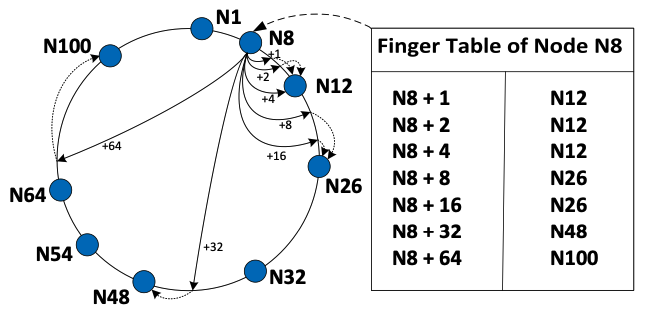
\includegraphics[width=.6\textwidth]{figures/chord-ring-network-sensor-nodes-finger-table.png}
     \rule{35em}{0.5pt}
    \caption{Chord ring network with sensor nodes and finger table in WiChord (\cite{balatsouras2022wichord})} 
\end{figure}


WiChord employs a \gls{dht}-based architecture similar to Chord but optimized for \glspl{wsn}.
It enables efficient data aggregation and query processing by minimizing communication overhead and conserving energy.
Nodes in WiChord aggregate data at intermediate points before forwarding it to the base station, reducing transmissions and extending network lifetime.
Additionally, WiChord optimizes routing paths and minimizes hops needed for data transmission, with nodes capable of entering low-power sleep modes to conserve energy further.
It maintains scalability and fault tolerance, handling the addition and failure of nodes without significant disruption.

\begin{figure}[htbp]
    \centering
 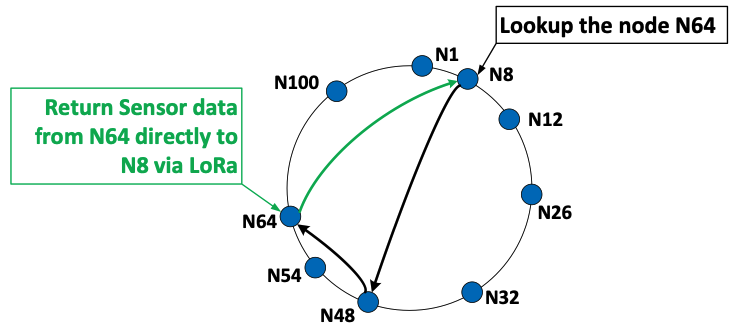
\includegraphics[width=.6\textwidth]{figures/chord-lookup-message-from-one-node-to-another.png}
     \rule{35em}{0.5pt}
    \caption{A lookup message from 2 nodes on a Chord sensor network nodes in WiChord (\cite{balatsouras2022wichord})} 
\end{figure}

WiChord can be applied in various real-world scenarios, including environmental monitoring, smart agriculture, and urban infrastructure monitoring.
For example, in environmental monitoring, WiChord efficiently collects and transmits data from dispersed sensor nodes to detect early signs of forest fires.
In smart agriculture, it supports precision farming by collecting and transmitting data on soil moisture and crop health, aiding farmers in making informed decisions.
In urban infrastructure monitoring, WiChord helps ensure timely maintenance of structures like bridges and buildings by collecting data on structural health indicators.

The primary advantages of WiChord are its energy efficiency, scalability, and robust data aggregation capabilities, making it suitable for long-term deployments in large-scale \glspl{wsn}.
However, the protocol's complexity can make implementation and maintenance challenging, and its performance may be affected by highly dynamic environments.

WiChord exemplifies how the principles of Chord can be adapted to address the specific needs of \glspl{wsn}, providing an efficient and scalable solution for various data aggregation and query processing applications.